\documentclass{article}
\usepackage{graphicx}
\usepackage{listings}
\usepackage{enumitem}
\usepackage{dingbat}
\usepackage{xcolor}
\usepackage{graphicx}
\usepackage{algpseudocode}
\usepackage{algorithm}
\usepackage[hidelinks]{hyperref}
\usepackage[italian]{babel}
\usepackage[fleqn]{amsmath}
\usepackage{caption}

\DeclareCaptionType{equ}[][]
\floatname{algorithm}{Codice}

\title{JPokeBattle}
\author{Leonardo Ganzaroli 1961846}
\date{Febbraio 2025}

\begin{document}

\maketitle

\tableofcontents
\listoffigures

\hypersetup{allcolors=black}

\newpage

\section{Descrizione generale}

\fontsize{12pt}{14pt}\selectfont

Il progetto da sviluppare può essere riassunto come: \vspace{5pt}

\raggedright
\textit{"Replicare il gameplay delle lotte all’interno dei videogiochi della serie
Pokémon, facendo riferimento alla prima generazione"}. \newline

Per una descrizione più specifica si può far riferimento alla seguente lista di funzionalità richieste per questo progetto.  \newline

\textit{(Quelle implementate sono segnate con un  {\color{green}\checkmark}, quelle implementate parzialmente invece con  {\color{yellow}\checkmark}) \newline}

\textbf{Specifiche richieste:}
\begin{itemize}

    \item Feature minime 

    \begin{itemize}
    \setlength\itemsep{1em}

        \item Implementare i 3 starter, le loro statistiche e le loro mosse base: {\color{green}\checkmark} 
        
            \begin{itemize}
                \item Bulbasaur → Ruggito e Azione
                \item Charmander → Ruggito e Graffio
                \item Squirtle → Colpocoda e Azione
            \end{itemize}
    
        \item Creare una GUI utilizzando Java Swing o JavaFX. {\color{green}\checkmark}
        
        \item Implementare le schermate classiche presenti in un videogioco: {\color{green}\checkmark}
        
                \begin{itemize}
                \item Menù principale
                \item Schermata di combattimento
                \item Schermata di "Game Over"
                \item \ldots
            \end{itemize}

        \item Far affrontare al giocatore una serie di lotte fino alla sua sconfitta. {\color{green}\checkmark}

    \end{itemize}

    \item Feature tipiche

        \begin{itemize}
        \setlength\itemsep{1em}
        
            \item Implementare tutte le mosse dei Pokémon scelti ignorando però i cambiamenti di stato. {\color{yellow}\checkmark}

            \item Preservare lo stato dei pokémon del giocatore nella serie di lotte. {\color{green}\checkmark}
            
            \item Implementare una schermata leaderboard che mantenga i 10 record migliori. {\color{green}\checkmark}
    
        \end{itemize}

    \item Feature extra

        \begin{itemize}
        \setlength\itemsep{1em}

        \item Implementare punti individuali e punti allenamento che migliorino le capacità dei pokémon sulla base delle vittorie. {\color{yellow}\checkmark}

        \item Implementare i meccanismi di passaggio di livello ed evoluzione dei Pokémon, incluso l’apprendimento di nuove mosse. {\color{yellow}\checkmark}

        \item Implementare animazioni, riproduzione di audio clip, ed altri effetti grafici. {\color{yellow}\checkmark}

        \item Implementare unit test del backend.

        \item Creare un Jar eseguibile.

        \item Implementare strategie per un comportamento “intelligente” degli avversari.

        \item Implementare una modalità di gioco testuale via terminale, selezionabile in alternativa alla GUI.

        \end{itemize}

    \vspace{5pt}

\end{itemize}

\textbf{Elementi implementati in modo parziale (in ordine):} \vspace{4pt}

\begin{itemize}

\item Le mosse che portano solamente a dei cambiamenti di stato, che applicano degli effetti continui o comunque "particolari" sono state ignorate.

\item I punti allenamento non sono stati implementati.

\item Il sistema dei livelli è presente ma non quello delle evoluzioni.

\item L'unica "animazione" presente è solamente un delay tra la scritta "Appare pokémon X", la comparsa dello sprite e la riproduzione del verso. Non sono presenti altri effetti grafici.

\end{itemize}

\section{Progetto sviluppato}

Questa sezione contiene una breve descrizione della struttura del progetto e dell'interfaccia grafica.
    
\vspace{10pt}

\subsection{GUI}
    
    L'interfaccia grafica si può suddividere in 5 parti, ognuna creata ad hoc:

    \subsubsection{Menù principale}

        La finestra che contiene il menù principale.

        \vspace{5pt}

        \begin{figure}[ht]
            \centering
            \makebox[\textwidth]{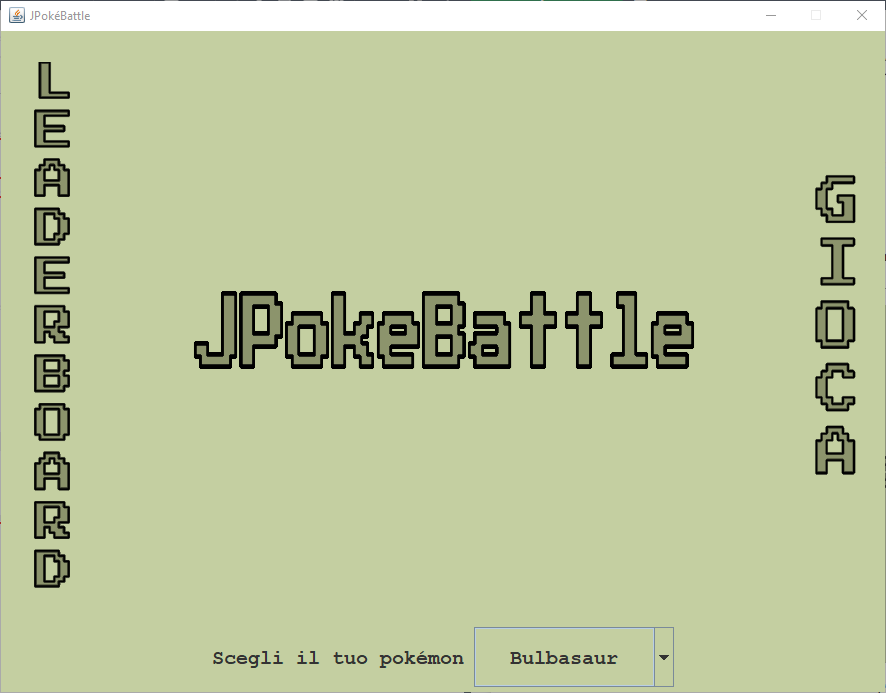
\includegraphics[width=.55\paperwidth]{Menu.png}}
            \caption{Menù}
            \label{fig:menu.png}
        \end{figure}

        Ai lati sono presenti 2 bottoni che permettono di aprire la Leaderboard (SX) e di giocare (DX). In basso è presente una combo box che permette di scegliere il pokémon da utilizzare.

    \subsubsection{Leaderboard}

        Contiene i migliori 10 record in termini di round vinti.

        \vspace{5pt}

        \begin{figure}[ht]
            \centering
            \makebox[\textwidth]{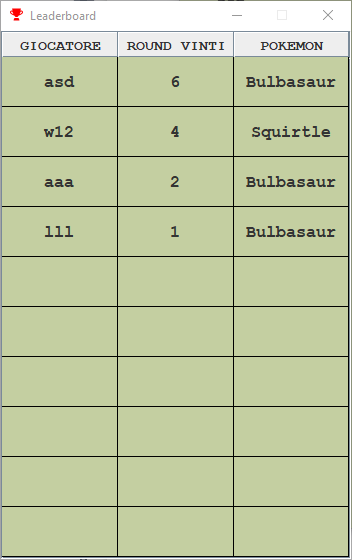
\includegraphics[width=.39\paperwidth]{Leaderboard.png}}
            \caption{Leaderboard con alcuni record}
            \label{fig:leaderboard.png}
        \end{figure}

    \newpage

    \subsubsection{Schermata di gioco}

        L'effettiva schermata di gioco, creata basandosi su quella dei vari giochi.

        \begin{figure}[h]
            \centering
            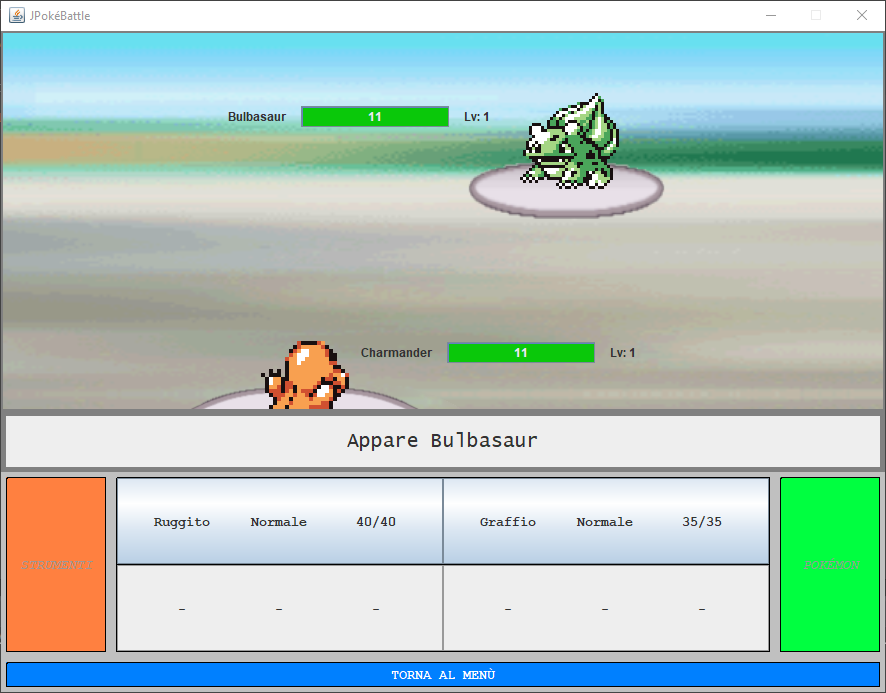
\includegraphics[width=\textwidth]{Gioco.png}
            \caption{Gioco appena avviato}
            \label{fig:gioco.png}
            \vspace{11pt}
            La parte inferiore della schermata andrà a variare con l'apprendimento di nuove mosse da parte del pokémon.\\
            \vspace{5pt}
            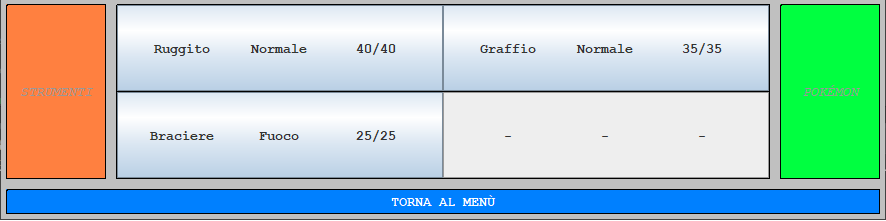
\includegraphics[width=.8\textwidth]{Gioco2.png}
            \caption{3 mosse}
            \label{fig:gioco2.png}
        \end{figure}

    \subsubsection{Game Over}

        Appare dopo la sconfitta del giocatore, nel caso in cui venga stabilito un nuovo record viene data la possibilità di salvarlo.

        \vspace{3pt}

        \begin{figure}[h]
            \centering
            \makebox[\textwidth]{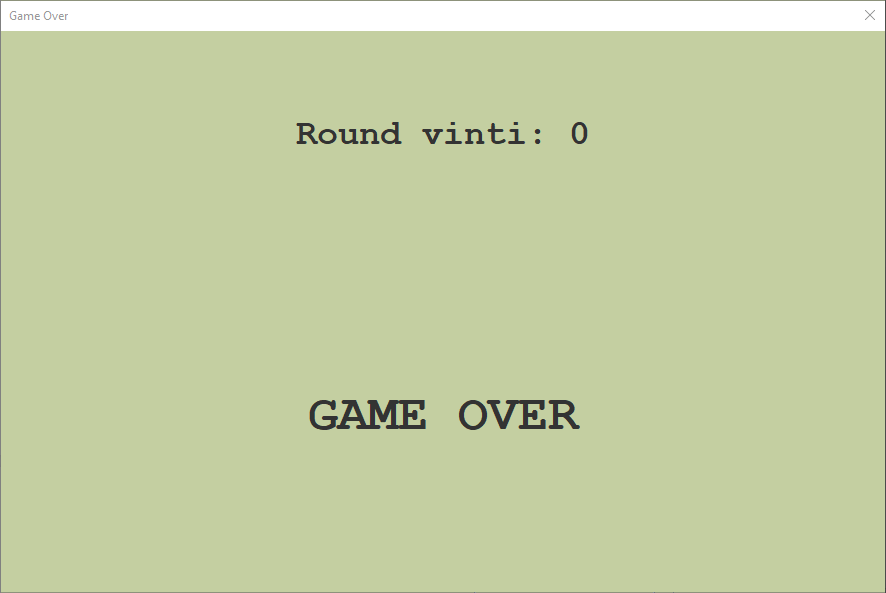
\includegraphics[width=.433\paperwidth]{GO.png}}
            \caption{No record}
            \label{fig:game_over.png}
        \end{figure}

        \begin{figure}[ht]
            \centering
            \makebox[\textwidth]{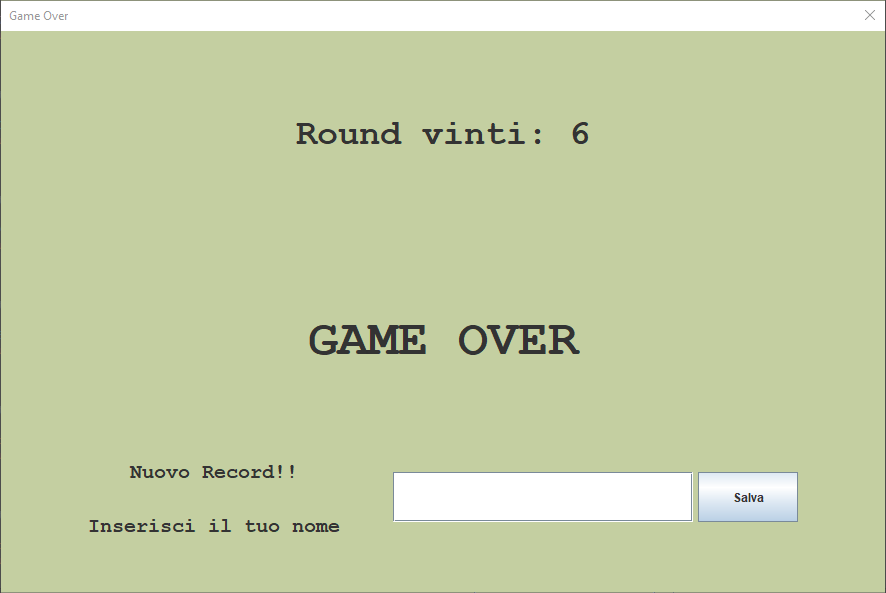
\includegraphics[width=.433\paperwidth]
            {GO2.png}}
            \caption{Nuovo record}
            \label{fig:game_over_record.png}
        \end{figure}

    \newpage

\vspace{5pt}

\subsubsection{Cambio mosse}

Usata quando il pokémon conosce già 4 mosse e vuole impararne una nuova, permette di scegliere se e quale mossa rimuovere.

\vspace{5pt}

        \begin{figure}[ht]
            \centering
            \makebox[\textwidth]{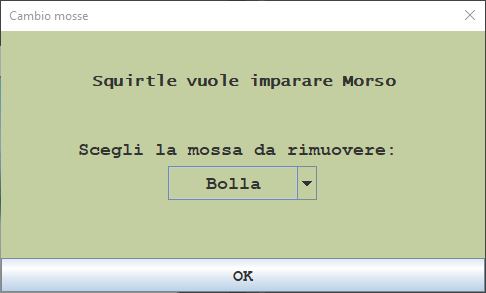
\includegraphics[width=.5\paperwidth]{Change.png}}
            \caption{Cambio mossa}
            \label{fig:change.png}
            \vspace{5pt}
        \end{figure}

In questo caso si sta rimuovendo Bolla per far imparare Morso.

\vspace{10pt}

\subsection{Struttura}

Per avere maggiore flessibilità viene fatto uso di file testuali contenenti tutte le informazioni riguardanti i pokémon e le loro mosse. In questo modo viene data la possibilità di creare/modificare i valori a piacimento rendendo possibile all'utente l'uso di elementi custom.

Per quanto riguarda le classi utilizzate e la loro struttura si identificano 3 elementi principali.

\newpage

\subsubsection{Pokémon}

La classe che rappresenta un pokémon, contiene le statistiche e le mosse in aggiunta a varie funzioni. Sono state inoltre create 2 sottoclassi per rappresentare il giocatore ed i nemici, ognuna con funzioni specifiche necessarie per il funzionamento del gioco.

\subsubsection{Statistiche}

La classe che raggruppa tutti i valori associati ad un certo pokémon: Vita, Attacco, Difesa, \ldots.

\subsubsection{Mosse}

Considerando i requisiti del progetto è stato possibile dividere ogni singola mossa in una di queste 5 categorie:

\begin{enumerate}
    \item Danneggia l'avversario

    \vspace{5pt}
    
    \begin{enumerate}
        \item Danni normali
        \item Danni speciali
    \end{enumerate}

    La formula usata per calcolare i danni è identica nei due casi ma i valori usati sono leggermente diversi.

    \vspace{3pt}

    \begin{equ}[!ht]
        \caption*{\href{https://bulbapedia.bulbagarden.net/wiki/Damage}{Formula della prima generazione:}}
    \begin{equation}
    \label{Formula_danno}
       \color{gray}\boxed{\color{black} \left( \frac{\left( \frac{2 \times Livello \times Critico}{5} + 2 \right) \times Potenza \times \left( \frac{A}{D} \right)}{50} + 2 \right) \times STAB \times Tipo1 \times Tipo2 \times Random}
        \nonumber
    \end{equation}
    \end{equ}
    
    \item Cambia le statistiche
    \begin{enumerate}
        \item Dell'avversario
        \item Proprie
    \end{enumerate}

    \item Mosse con effetti particolari
\end{enumerate}

\vspace{3pt}

L'ultimo tipo è stato inserito per permettere di creare eventuali mosse che non rientrano nelle altre categorie, in questo modo c'è la possibilità di aggiungere quelle non implementate in futuro (vedere sezione successiva). 

\newpage

\subsection{Design Pattern}

In questo progetto sono presenti 2 pattern.

\vspace{5pt}

\subsubsection{Strategy}

Per implementare le mosse è stato utilizzato il pattern Strategy, in questo modo si potrà scegliere la funzione più adatta da associare ad una certa mossa. Permette inoltre di creare ulteriori funzioni in caso di necessità. 

    \begin{figure}[ht]
        \centering
        \makebox[\textwidth]{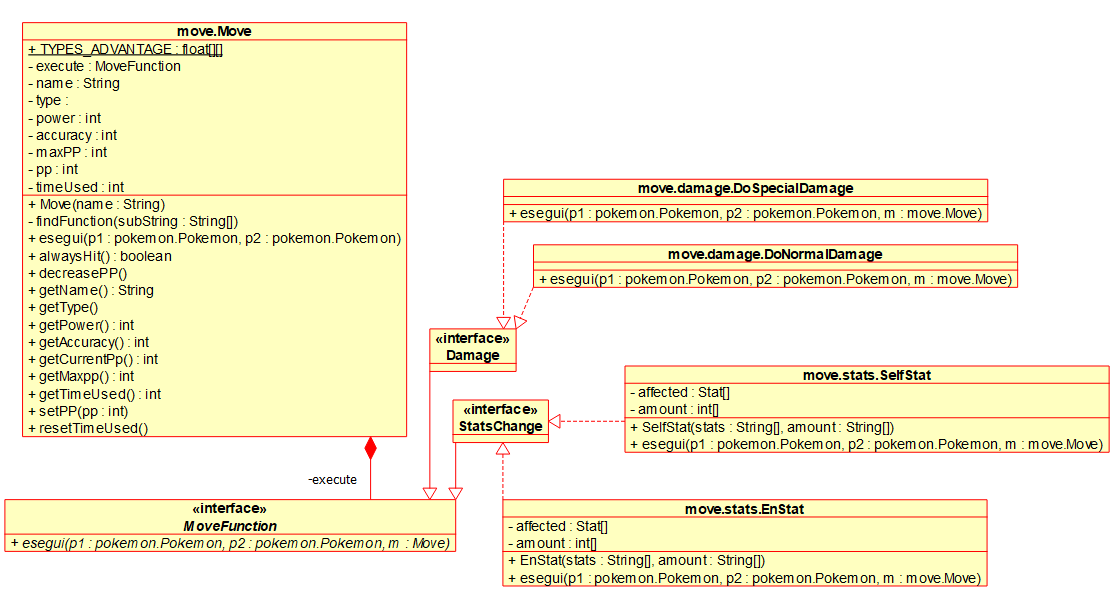
\includegraphics[width=.95\paperwidth]{Strategy.png}}
        \caption{Strategy pattern}
        \label{fig:strategy.png}
    \end{figure}

\newpage

\subsubsection{Singleton}

Dato che la leaderboard è una finestra a sè stante apribile dal menù viene utilizzato il pattern Singleton per evitare l'apertura di finestre multiple.

    \begin{figure}[ht]
        \centering
        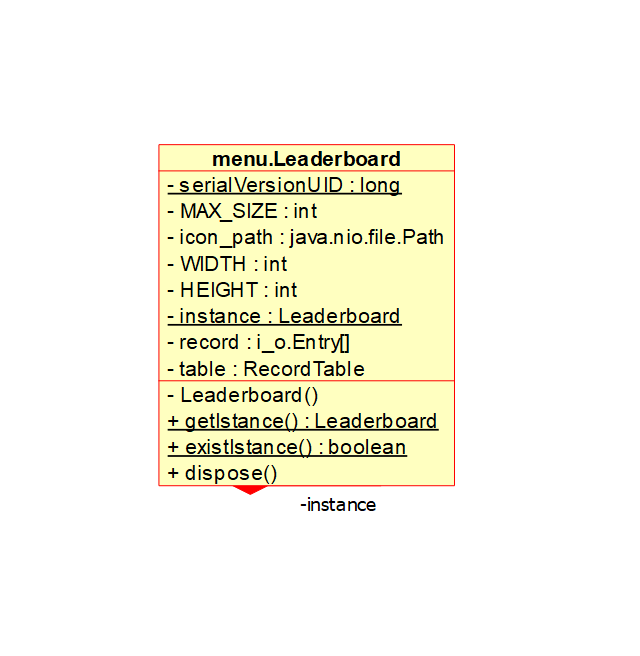
\includegraphics[width=\textwidth]{Singleton.png}
        \caption{Singleton pattern}
        \label{fig:singleton.png}
    \end{figure}

\newpage

\subsection{Paradigmi di programmazione}

\vspace{5pt}

\subsubsection{Stream}

Sono presenti 2 funzioni nel codice in cui si fa uso degli stream, entrambe hanno a che fare con la lettura di file testuali: \newline\textbf{(N.B. br è il BufferedReader)}

\vspace{5pt}
\begin{enumerate}
    \item Nella funzione \textit{allPokemon} della classe \textit{FileRw}, dove è presente la seguente riga: 
    \begin{algorithm}
    \label{alg:str1}
    \caption{Crea un insieme contenente tutti i nomi dei pokémon presenti nel file.}
    \begin{algorithmic}[ht]
    \Statex $result = br.lines()$ 
    \State\hspace{\algorithmicindent}$.filter(x $→$ x.contains("name:"))$
    \State\hspace{\algorithmicindent}$.map(x $→$ x.replace("name:",""))$
    \State\hspace{\algorithmicindent}$.collect(Collectors.toCollection(TreeSet::new));$
    \end{algorithmic}
    \end{algorithm}

    \vspace{5pt}

\item Nel ciclo della funzione \textit{fill} della classe \textit{Entry}:
    \begin{algorithm}
    \label{alg:str2}
    \caption{Legge i record dal file e crea un array di oggetti Entry che verranno poi utilizzati nel ciclo.}
    \begin{algorithmic}[ht]
    	\For{$(Entry$ $e : br.lines()$
        \State\hspace{\algorithmicindent}$.filter(x $→$ !x.isEmpty())$
        \State\hspace{\algorithmicindent}$.map(x $→$ new $ $ Entry(x.split("$ $")))$
        \State\hspace{\algorithmicindent}$.sorted(Comparator.comparing(Entry::getStreak).reversed())$
        \State\hspace{\algorithmicindent}$.limit(MAX\_RECORD)$
        \State\hspace{\algorithmicindent}$.toArray(Entry[]::new))$} 
        \State ${\ldots}$
        \EndFor
    \end{algorithmic}
    \end{algorithm}
    
\end{enumerate}

\end{document}